\documentclass[11pt,final,reqno]{amsart}
\addtolength{\textheight}{0.5in}
\addtolength{\topmargin}{-0.2in}
\addtolength{\oddsidemargin}{-.45in}
\addtolength{\evensidemargin}{-.45in}
\addtolength{\textwidth}{1.0in}

\renewcommand{\baselinestretch}{1.04}

\usepackage{bm,url,xspace,fancyvrb}
\usepackage{amssymb,amsmath}
\usepackage[final,pdftex]{graphicx}
\usepackage[pdftex, colorlinks=true, plainpages=false, linkcolor=blue, citecolor=red, urlcolor=blue]{hyperref}
\pdfinfo{ /Title (Numerical solution of the Blatter stress balance for glacier flow)
          /Author (Ed Bueler) } 

\newtheorem*{thm}{Theorem}

\theoremstyle{remark}
\newtheorem*{fiction}{Fiction}

\theoremstyle{definition}
\newtheorem*{defn}{Definition}

\newcommand{\ddt}[1]{\ensuremath{\frac{\partial #1}{\partial t}}}
\newcommand{\ddx}[1]{\ensuremath{\frac{\partial #1}{\partial x}}}
\newcommand{\ddy}[1]{\ensuremath{\frac{\partial #1}{\partial y}}}
\newcommand{\pp}[2]{\ensuremath{\frac{\partial #1}{\partial #2}}}
\newcommand{\eps}{\epsilon}
\newcommand{\grad}{\nabla}

\newcommand{\CC}{\mathbb{C}}
\newcommand{\RR}{\mathbb{R}}
\newcommand{\ZZ}{\mathbb{Z}}

\newcommand{\bbF}{\mathbf{F}}
\newcommand{\bG}{\mathbf{G}}
\newcommand{\bU}{\mathbf{U}}
\newcommand{\bY}{\mathbf{Y}}

\newcommand{\bb}{\mathbf{b}}
\newcommand{\bs}{\mathbf{s}}
\newcommand{\bw}{\mathbf{w}}

\newcommand{\nue}{{\nu^\eps}}
\newcommand{\nuek}{{\nu_k^\eps}}

\newcommand{\HoneX}[1]{\mathcal{H}_{#1}(\Omega)}
\newcommand{\Hone}{\HoneX{}}
\newcommand{\HoneD}{\HoneX{D}}
\newcommand{\Honezero}{\HoneX{0}}

\newcommand{\WonepX}[1]{\mathcal{W}^{1,p}_{#1}(\Omega)}
\newcommand{\Wonep}{\WonepX{}}
\newcommand{\WonepD}{\WonepX{D}}
\newcommand{\Wonepzero}{\WonepX{0}}
\newcommand{\X}{\mathcal{X}}
\newcommand{\XD}{\mathcal{X}_D}
\newcommand{\Xzero}{\mathcal{X}_0}

\newcommand{\TESTONE}{\texttt{TEST1}\xspace}
\newcommand{\TESTTWO}{\texttt{TEST2}\xspace}

\newcommand{\Matlab}{\textsc{Matlab}\xspace}
\newcommand{\Octave}{\textsc{Octave}\xspace}

\begin{document}

\title[Numerical solution of the Blatter stress balance]{Numerical solution of the \\ Blatter stress balance for glacier flow}
\author{Ed Bueler}
\date{\today}

\begin{abstract}
These notes are an extended, constructive tutorial on computing the velocity field which solves the Blatter model for glacier flow \cite{Blatter,ColingeRappaz,Pattyn03} in a two-dimensional flowline geometry.  Functional \Matlab/\Octave codes which implement a finite element model \cite{Elmanetal2005} are constructed.  There is no attempt to derive the model, because reference \cite{SchoofHindmarsh}, among others, covers this.  By reading these notes the reader should learn:
\begin{itemize}
\item what is the weak form of the Blatter equation,
\item how to construct a finite element method based on quadrilaterals,
\item how to use Newton's method to generate a rapidly-convergent sequence of numerical approximations to the solution of the nonlinear model,
\item how to adequately verify the linear, nonlinear, and boundary condition components of the numerical implementation, and
\item the amount by which the Blatter solution differs from the SIA solution in the non-sliding case.
\end{itemize}
This tutorial also serves as an introduction to a new three-dimensional, parallel-scalable Blatter solver in \cite{BrownSmithAhmadia2013}.
\end{abstract}

\maketitle

\setcounter{tocdepth}{1}
\tableofcontents
\vfill


\newpage
\section{Continuum model}\label{sec:continuum}

\subsection*{Equation for horizontal velocity}  Our eventual goal is to approximate (compute) the velocity solution of a certain stress balance for glacier flow, the Blatter model \cite{Blatter,ColingeRappaz,Pattyn03,SchoofCoulombBlatter,SchoofHindmarsh}.  First we consider the continuum model and then we address the finite element approximation at some length.  Though the presentation is largely self-contained, the reader who has references \cite{Elmanetal2005} and \cite{SchoofHindmarsh} at hand will be most efficient.

The Blatter model includes all the physics in the simpler SIA or SSA models \cite{SchoofHindmarsh}, but like them it is a \emph{shallow} approximation of ice flow.  All of these models come from small-aspect ratio limits of the Stokes model \cite{Fowler,SchoofHindmarsh}, but both the SIA and the SSA models are derivable from the Blatter model by further small-parameter limits \cite{SchoofHindmarsh}.  These facts suggest, but do not demonstrate in any particular setting, the superior flow approximation of the Blatter model relative to shallower models.  The Blatter model is described in one textbook \cite[subsection 5.3]{GreveBlatter2009} as a shallow approximation of the somewhat more general ``hydrostatic'' model, which is itself an approximation of the Stokes model.

The glacier model here is a plane, the flow line geometry which is shown in Figure \ref{fig:profile}, with surface $z=h(x)$, base $z=b(x)$, and horizontal extent $0<x<L$.

We assume the ice is at a single temperature (isothermal) and that there is no slip (sliding) at its base.  The model is, however, still complete enough to study the effect of basal topography on the velocity field solving the Blatter model.  Improved modeling of flow over irregular bed geometry is one important reason to remove shallowness assumptions by using the Blatter model instead of shallower models (e.g.~SIA or SSA or hybrids thereof \cite{BBssasliding,Goldberg2011}).

In these notes we will not consider the Blatter model coupled to the mass continuity equation, so we are addressing the instantaneous velocity field arising from the boundary stresses and body forces (gravity), and we do not consider how the geometry might change.

We seek a velocity solution with components $u=u(x,z)$, $w=w(x,z)$ within the region shown in Figure \ref{fig:profile} in a plane with coordinates $(x,z)$.  The Blatter model, and the SIA and SSA also, allow us to compute the horizontal component $u$ without explicit attention to the other component $w$.  As described in section \ref{sec:sia}, once $u$ is known an integral computes $w$ using incompressibility.

\begin{figure}[ht] 
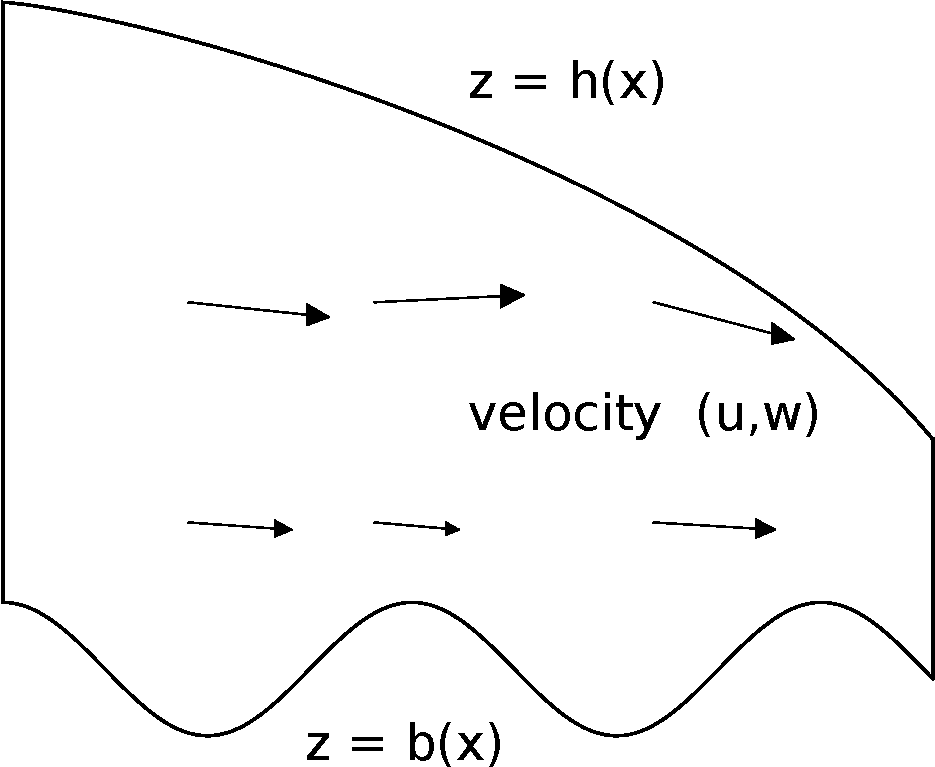
\includegraphics[width=0.45\textwidth]{figs/profile}
\caption{Profile of a flow line in an ice sheet.  We will compute the velocity solution $(u,w)$ of equation \eqref{blatter} in this region.}
\label{fig:profile}
\end{figure}

We suppose that ice flows according to the Glen constitutive relation \cite[equation (4.16)]{GreveBlatter2009}
\begin{equation}
  D_{ij} = A_0 \tau^{n-1} \tau_{ij}.  \label{glen}
\end{equation}
Here $D_{ij}$ is the strain rate tensor, a symmetric matrix (tensor) of derivatives of the velocity field.  It is a $2\times 2$ matrix in our flowline case:
	$$D_{ij}=\begin{pmatrix} u_x & \frac{1}{2}\left(u_z+w_x\right) \\
	                                     \frac{1}{2}\left(u_z+w_x\right) & w_z\end{pmatrix}.$$
In equation \eqref{glen}, $n > 1$ is the Glen exponent, $\tau_{ij}$ is the deviatoric stress tensor \cite{GreveBlatter2009}, and the relation $2 \tau^2 = \tau_{ij}\tau_{ij}$ defines the ``effective deviatoric stress'' $\tau$, also known as the second invariant of the tensor $\tau_{ij}$.  Equation \eqref{glen} may be written as an equivalent viscosity relation \cite[equation (4.22)]{GreveBlatter2009}
\begin{equation*}
  \tau_{ij} = 2 \nu D_{ij} \qquad \text{ where } \qquad \nu = \frac{B_0}{2} D^{(1-n)/n}.
\end{equation*}
Again $2 D^2 = D_{ij} D_{ij}$ defines the effective strain rate.  Note $A_0>0$ is the ice ``softness'' and $B_0=A_0^{-1/n}$ is the ice hardness; both are constant in this paper by our isothermal assumption.

The Blatter stress balance model is a single PDE for the horizontal velocity component $u$:
\begin{equation}
\left(4 \nu u_x\right)_x + \left(\nu u_z\right)_z = \rho g h'.\label{blatter}
\end{equation}
To derive equation \eqref{blatter} from the published 3D form of the Blatter model---for example equation (15) in \cite{Pattyn03}, equation (2.1a) in \cite{SchoofCoulombBlatter}, or equation (5.70) in \cite{GreveBlatter2009}---remove all cross-flow derivatives (i.e.~``$\partial/\partial y=0$'') and cross-flow velocities (i.e.~``$v=0$'').

By its definition above, the effective strain rate $D$ satisfies $D^2 = u_x^2 + (1/4)\left(u_z + w_x\right)^2.$  In the Blatter model there is, however, the additional approximation $|w_x| \ll |u_z|$ (see \cite{GreveBlatter2009,Pattyn03}).  It follows that the viscosity takes the form
\begin{equation}
\nu = \frac{B_0}{2} \left(u_x^2 + \frac{1}{4}u_z^2\right)^{(1-n)/(2n)}. \label{visc}
\end{equation}
The nonlinear elliptic PDE of the Blatter model arises from substituting equation \eqref{visc} into equation \eqref{blatter}.  Thus we may compute the ice viscosity given strain rates $u_x$ and $u_z$.  The power in \eqref{visc} is negative, however, and if all strain rates are zero then the resulting viscosity is infinite.  This well-known issue has a well-known solution, namely \emph{regularization} \cite{Pattyn03,SchoofCoulombBlatter}.  We treat regularization here as part of the numerical solution, in that we will eventually examine how the method behaves when we reduce the value of the regularization parameter toward its no-regularization limit.\footnote{It is also possible to treat the issue as one of physics, as in subsection 4.3 of \cite{GreveBlatter2009}.}  As a default value, let $\eps_0$ be the strain rate of 1 m/a velocity change in 100 km, so $\eps_0 = 3.1689 \times 10^{-13} \,\text{s}^{-1}$ in MKS units.  The regularized viscosity is defined
\begin{equation}
\nu = \nu(u_x,u_z) = \frac{B_0}{2} \left(u_x^2 + \frac{1}{4}u_z^2 + \eps_0^2\right)^{(1-n)/(2n)}. \label{viscreg}
\end{equation}
From now on, by mild abuse of notation, ``viscosity'' $\nu$ refers to this regularized form.  

\subsection*{Boundary conditions}  The continuum model is obviously not complete without boundary conditions.  Said positively, Schoof \cite{SchoofCoulombBlatter} shows that equation \eqref{blatter} is part of a well-posed model for the velocity field if one supplies boundary conditions like those we now state, but also including standard sliding laws.  

\begin{figure}[ht] 
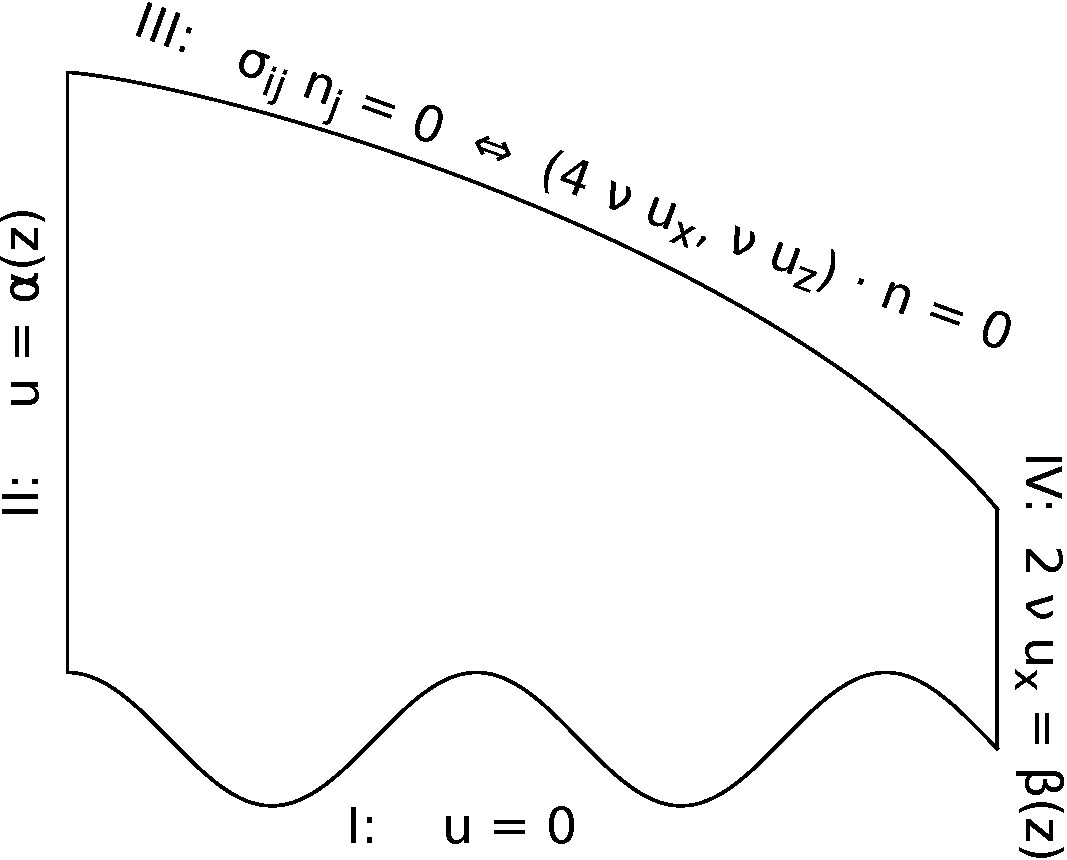
\includegraphics[width=0.50\textwidth]{figs/bdryblatter}
\caption{Boundary conditions for our Blatter model.}
\label{fig:bdryblatter}
\end{figure}

For the present example we impose particular boundary conditions shown in Figure \ref{fig:bdryblatter}.  We describe these in clockwise order, starting at the base of the ice:
\renewcommand{\labelenumi}{\Roman{enumi}.\quad}
\begin{enumerate}
\item Along its base $z=b(x)$ the ice is not slipping, so $u=0$.
\item At the upstream (left) end on the vertical line $x=0$ we impose a known (pre-determined) ice velocity $u=\alpha(x)$.  For example, $u = 0$ for all $z$ at $x=0$ corresponds to the upstream end being located at a divide, which is what we will choose for our concrete example.
\item On the upper surface $z=h(x)$ there is a normal-stress-balance boundary condition $\sigma_{ij} n_j = 0$, where $\sigma_{ij}$ is the Cauchy (full) stress tensor and $n_j$ is a normal to the upper surface.  Appendix A shows that, based on the scalings in \cite{SchoofHindmarsh}, and up to the same size of shallow-approximation error made in the rest of the Blatter model, this boundary condition is equivalent to a ``natural'' Neumann condition for \eqref{blatter}:
\begin{equation}
   \sigma_{ij} n_j = 0 \quad \iff \quad (4 \nu u_x, \nu u_z) \cdot \mathbf{n} = 0. \label{upper}
\end{equation}
Because $\mathbf{n}=(-h',1)$ is a normal vector on the upper surface and $\nu >0$, the condition can also be written $-4 h' u_x + u_z = 0$.
\item At the downstream end $z=L$ we suppose there is a pre-determined longitudinal (normal) stress which may depend on the vertical coordinate, thus:
\begin{equation}
2 \nu u_x = B_0 \left(u_x^2 + \frac{1}{4}u_z^2\right)^{(1-n)/(2n)} u_x = \beta(z). \label{downstream}
\end{equation}
The condition adopted for the calving front in a vertically-integrated SSA model, namely $u_x = [(1 - \rho/\rho_w) \rho g H / (4 B_0) ]^n$ \cite{GreveBlatter2009}, which we will choose for our concrete example, is one specific case which fits into form \eqref{downstream}.
\end{enumerate}

The basal (I) and upstream (II) boundaries together form the Dirichlet component of the boundary.  The upper surface (III) and the downstream (IV) boundary together form the Neumann component.  Based on a Poisson equation analog \cite[i.e.~the equation $u_{xx}+u_{yy}=f$]{Ockendonetal2003}, for example, we expect equation \eqref{blatter} with these boundary conditions to have a unique solution.  This is proven in \cite{RappazReist05,SchoofCoulombBlatter}.

\subsection*{Linearized weak form}  Denote the region in which we seek the horizontal velocity $u$ by
\begin{equation}
	\Omega = \left\{(x,z) \,\Big|\, 0<x<L, \, b(x) < z < h(x)\right\}. \label{domain}
\end{equation}
The solution $u(x,z)$ of equation \eqref{blatter} must be a function which is differentiable on $\Omega$, but we leave the exact degree of smoothness undetermined for a moment.  We will build a finite element solution based on the idea that the ``strong'' equation \eqref{blatter} implies that certain integrals over $\Omega$ are zero.  These integrals are the ``weak-form'' of the equation, which uses infinitely-many ``test functions'' in its integrals.  In the finite element method, test functions are constructed from a mesh on $\Omega$, and finitely-many of these will determine the finite element solution.

This section and the next two subscribe to a linearization ``fiction,'' however, which simplifies the initial construction of a numerical method.  In section \ref{sec:nonlinear} we remove the fiction and address the fully-nonlinear Blatter equation.

\begin{fiction}  We suppose the viscosity $\nu=\nu(x,z)$ is a known, positive, and smooth function of $x,z$, which is bounded above and below by positive constants, $0 < \nu_1 \le \nu(x,z) \le \nu_2$.
\end{fiction}

We know that the actual Blatter equation \eqref{blatter} incorporates the Glen law for ice, wherein the viscosity depends on derivatives of velocity, so the left side of equation \eqref{blatter} depends nonlinearly on $u$.  The assumption that the viscosity is bounded below turns out to be both important and justified, however.  Indeed, the viscosity regularization in equation \eqref{viscreg} implies that $\nu \ge  \eps_0^{(1-n)/n} > 0$ for the full nonlinear problem.

Recall the divergence theorem for $\Omega$: if $\mathbf{X}=(a,b)$ is a vector field on $\Omega$ and $\mathbf{n}$ is an outward unit normal along the boundary curve $\partial\Omega$ then
\newcommand{\dxdz}{\;\mathrm{d}x\,\mathrm{d}z} 
	$$\int_\Omega \nabla\cdot \mathbf{X} \dxdz = \int_\Omega a_x + b_z \dxdz = \int_{\partial\Omega} \mathbf{X}\cdot \mathbf{n}\,\mathrm{d}s.$$
The symbols ``$\int_{\partial\Omega} \mathrm{d}s$'' denote integration along $\partial\Omega$ using arclength parameterization.  Recall also the product rule for a scalar function $f$ and a vector field $X$,
	$$\nabla\cdot \left(f \mathbf{X}\right) = \nabla f\cdot \mathbf{X} + f \nabla\cdot \mathbf{X}.$$

The product rule and the divergence theorem together allow us to integrate by parts on $\Omega$.  In fact, let $\varphi(x,z)$ be a differentiable function on $\Omega$; we defer for a moment any precise statements about smoothness.  Multiplying both sides of equation \eqref{blatter} by $\varphi$, then using the above product rule, and then using the divergence theorem gives this calculation:
\begin{align*}
    \int_\Omega \Big[\left(4 \nu u_x\right)_x + \left(\nu u_z\right)_z\Big]\,\varphi \dxdz &= \int_\Omega \rho g h'\,\varphi \dxdz, \\
    \int_\Omega \nabla \cdot \Big((4 \nu u_x,\nu u_z) \varphi\Big)\dxdz - \int_\Omega (4 \nu u_x,\nu u_z) \cdot \nabla \varphi \dxdz &= \int_\Omega \rho g h'\,\varphi \dxdz, \\
    \int_{\partial\Omega} \varphi(4 \nu u_x, \nu u_z) \cdot \mathbf{n}\,\mathrm{d}s - \int_\Omega \nu (4 u_x, u_z) \cdot \nabla \varphi \dxdz &= \int_\Omega \rho g h'\,\varphi \dxdz.
\end{align*}

With the boundary conditions described earlier (Figure \ref{fig:bdryblatter}), the boundary integral can be decomposed into four parts.  Two of these parts have Dirichlet boundary conditions, so we assume
	$$\varphi(x,z) \text{ is zero along parts I and II of } \partial \Omega.$$
On part III we have $(4 \nu u_x, \nu u_z) \cdot \mathbf{n} = 0$, while on part IV, where $\mathbf{n} = (1,0)$, and using equation \eqref{downstream}, we have $(4 \nu u_x, \nu u_z) \cdot \mathbf{n} = 4 \nu u_x = 2\beta(z)$.  Thus the integrals along three of the four parts of $\partial\Omega$ give zero, and the remaining part no longer involves unknown $u$.  Rearranging the last equation gives
\begin{equation}
\int_\Omega \nu (4 u_x, u_z) \cdot \nabla \varphi \dxdz = - \int_\Omega \rho g h'\,\varphi \dxdz + \int_{\mathrm{IV}} 2 \beta \varphi \,\mathrm{d}z.  \label{weakearly}
\end{equation}
Equation \eqref{weakearly} is, already, the linearized weak form of the Blatter equations, but we need to be a bit clearer on functions spaces and boundary conditions.  Note only first derivatives $u_x,u_z$ appear in equation \eqref{weakearly}.  Note that test functions are assumed to satisfy Dirichlet conditions on parts of the boundary in different ways.

\begin{defn}  Recall that $L^2(\Omega)$ denotes the space of all functions $f : \Omega \to \RR$ which are square-integrable on $\Omega$.  The Sobolev space\footnote{The textbook by Elman and others \cite{Elmanetal2005} glosses the relevant function space theory.  A more serious PDE textbook like Evans \cite{Evans} provides more precision.} for our linearized equation is a subspace of  $L^2(\Omega)$,
	$$\Hone = \left\{f:\Omega \to \RR \,\Big|\, f,f_x,f_y \in L^2(\Omega)\right\}.$$
The \emph{solution (trial)} space $\HoneD$ and \emph{test} space $\Honezero$ are subsets of $\Hone$, namely
\begin{align}
     \HoneD &= \left\{f \in \Hone \,\Big|\, f|_{I} = 0, f|_{II} = \alpha(x)\right\}, \label{solntestspaces} \\
  \Honezero &= \left\{f \in \Hone \,\Big|\, f|_{I} = 0, f|_{II} = 0\right\}. \notag
\end{align}
\end{defn}

We can now state the weak form of the linearized Blatter equation precisely.

\begin{defn}
A function $u=u(x,z)\in\HoneD$ \emph{solves the linearized weak form} for fixed viscosity field $\nu=\nu(x,z)$ of equation \eqref{blatter} if
\begin{equation}
\int_\Omega \nu\, (4 u_x, u_z) \cdot \nabla \varphi \dxdz = - \int_\Omega \rho g h'\,\varphi \dxdz + \int_{\mathrm{IV}} 2 \beta \varphi \,\mathrm{d}z \label{weak}
\end{equation}
for all $\varphi=\varphi(x,z)\in\Honezero$.
\end{defn}

The upper surface III makes no explicit appearance in the integrals in \eqref{weak}, nor in the construction of the solution or test spaces.  Thus so-called ``natural'' boundary conditions apply there.  Also notice that the solution $u\in \HoneD$ and the test functions $\varphi \in \Honezero$ are in distinct spaces if $\alpha(z)\ne 0$ along boundary component II.

The weak form states infinitely-many facts about $u$, because \eqref{weak} holds for each of the infinitely-many test functions $\varphi$.  On the other hand, we could also say that equation \eqref{blatter} applies at infinitely-many points, at each $(x,z)\in \Omega$.  In any case, it is known that the weak form is a ``good'' mathematical problem, because it actually has a solution and only one solution in rather general circumstances.\footnote{Proofs for the fully-nonlinear Blatter problem are in \cite[theorem 2.1]{RappazReist05} and \cite[theorem 4.2]{SchoofCoulombBlatter}.}  The derivation above shows that a strong solution (of \eqref{blatter}) is also a weak solution (of \eqref{weak}).  The weak form can, however, have a unique solution which is not smooth enough to make sense of the derivatives in the strong form \cite{Evans}.  The three-dimensional weak form of the Blatter equations appears in \cite{BrownSmithAhmadia2013} and \cite{SchoofCoulombBlatter}.

The weak form is used to construct finite element approximations (next section), in contrast with finite difference methods which discretize the strong form.  As already said, in the finite element method we will generate algebraic equations from equation \eqref{weak} using a finite list of test functions $\varphi$ generated from a mesh on $\Omega$.  In section \ref{sec:nonlinear} we return to the (continuum) weak form and state it correctly for the fully nonlinear, viscosity-regularized Blatter equation.


\newpage
\section{Numerical approximation using \texorpdfstring{$Q_1$}{Q\textonesuperior} finite elements}\label{sec:fem}  % idiotic: \textoneinferior not defined for me

\subsection*{Mesh}   Our mesh will be a logically-rectangular grid, with $I$ intervals in the horizontal and $J$ vertical levels.  Consider the curves
\begin{equation}
	z_j(x) = b(x) + \frac{j^\gamma}{J^\gamma} (h(x) - b(x)) \label{curves}
\end{equation}
for $j=0,1,\dots,J$ and $\gamma=0$.  These are shown in Figure \ref{fig:conform}.  These curves conform to the geometry of our glacier flow problem, and, for $\gamma>1$, they are concentrated near the base of the ice where there is generally more shearing flow.

\begin{figure}[ht] 
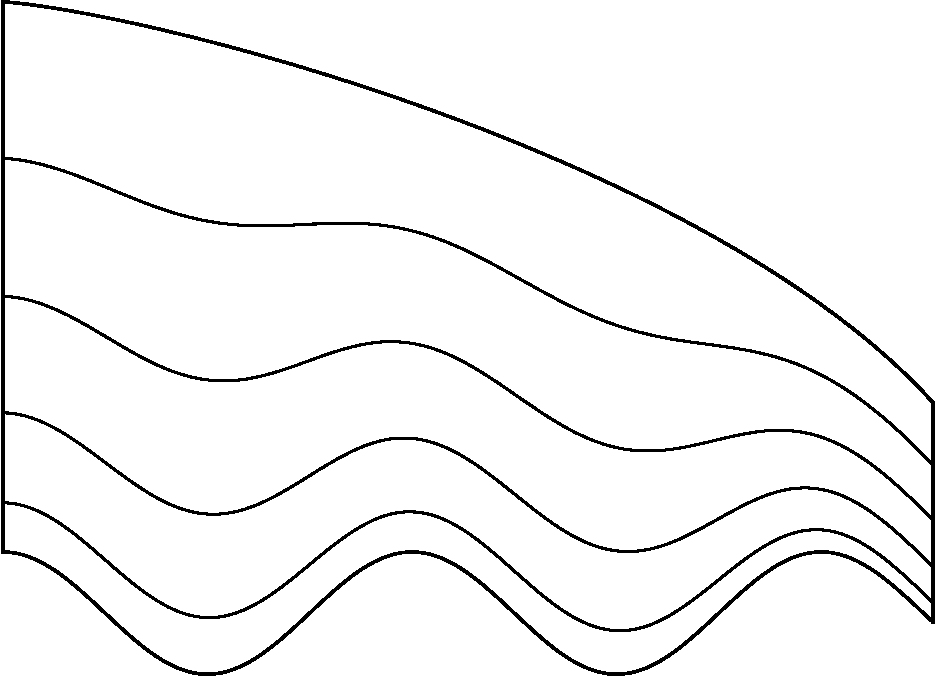
\includegraphics[width=0.5\textwidth]{figs/conform}
\caption{Curves $z=z_j(x)$ from equation \eqref{curves} for $J=5$ and $\gamma=1.5$.  Note $z_0(x)=b(x)$ and $z_J(x)=h(x)$.}
\label{fig:conform}
\end{figure}

In each column of ice (fixed $x$) these curves determine an unequally-spaced grid $\{z_j\}$.  Indeed, choose $I$ equal spaces in the $x$ direction and define spacing $\Delta x=L/I$.  For $i=0,\dots,I$, let $x_i = i \Delta x$.  The $N = (I+1)(J+1)$ nodes 
	$$(x_i,z_j(x_i))$$
determine a mesh shown in Figure \ref{fig:q1mesh}.  The mesh decomposes the domain into $I J$ quadrilaterals, which we call ``quads'' for short.  An approximation occurs already, because we have replaced the upper and lower curves $z=h(x)$ and $z=b(x)$ by polygonal approximations.  An increase in horizontal resolution (larger $I$) will improve the meshed approximation of bed features described by $z=b(x)$.
 
\begin{figure}[ht] 
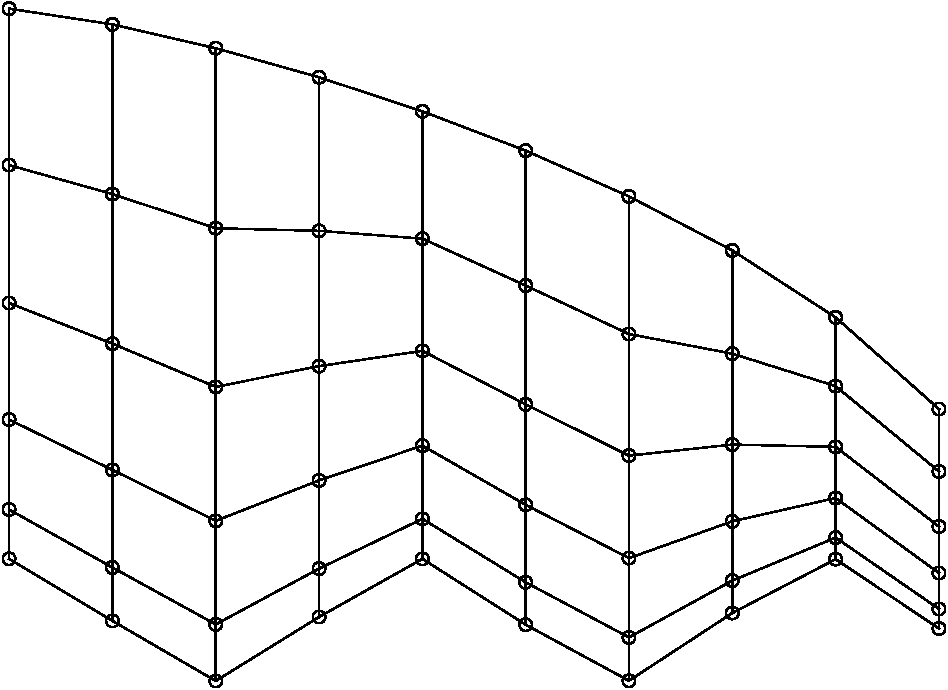
\includegraphics[width=0.5\textwidth]{figs/q1mesh}
\caption{Quadrilateral mesh with $I=9$ and $J=5$.  $N=60$ nodes.}
\label{fig:q1mesh}
\end{figure}

In the numerical method we number the nodes globally $n=1,2,\dots,N$.  The nodes correspond to approximate values $U_n$ of the velocity $u$ in equation \eqref{blatter}.  We also define node-location functions $i(n)$ and $j(n)$ so that the $n$th velocity unknown $U_n$ is at $\left(x_{i(n)},z_{j(n)}(x_{i(n)})\right)$ in the $x,z$ plane.  In particular, if $\lfloor \alpha\rfloor$ is the integer part of a real number $\alpha$ then $i(n) = \left\lfloor (n-1)(J+1) \right\rfloor$ and $j(n) = n - 1 - i(n)(J+1)$.  (This is easily checked by a few specific cases.  Note $j(n)$ is one less than the remainder after dividing $n$ by $J+1$.)  The inverse function to these node location functions is
\begin{equation}
  n(i,j) = i(J+1) + j + 1  \label{localtoglobal}
\end{equation}
for $i=0,\dots,I$ and $j=0,\dots,J$.  We will use the function $n(i,j)$ in many places in the numerical method, while the functions $i(n)$, $j(n)$ are typically only used for diagnosis, for example in determining which is the node that generated a certain equation in a linear system.

Thus the grid is \emph{structured} although the quads have variable geometry.  When we iterate over quads to assemble the matrix of the discretized Blatter equations we actually iterate over local grid indices $i,j$.  On the one hand, entries in the rows and columns of the matrix are modified according to the node numbers $n=n(i,j)$ computed from local grid indices.  On the other hand, during assembly of the linear system we will know from $i,j$, the node indices of the lower-left corner of the quad, what are the local and thus global indices of the other corner nodes for that quad.  Generally we will traverse corners of a quad starting at the lower-left and going counter-clockwise, thus $(i,j),\,(i+1,j),\,(i+1,j+1),\,(i,j+1)$.  By contrast, for an unstructured quadrilateralization or triangulation we would index the quads themselves and build a connectivity matrix relating quad index to the global node numbers of the vertices of the quad; see subsection 1.4.3 of \cite{Elmanetal2005}.

\newcommand{\quadij}{\square_{ij}}
\newcommand{\quadref}{\square_{\ast}}

\subsection*{Finite elements}  In the remainder of this section we follow the Elman and others \cite{Elmanetal2005}, when possible, in building a finite element method, but the presentation is largely self-contained.

Our method uses ``isoparametric'' quads (i.e.~same parameters).  Denote each quad in the mesh by
\begin{equation}
	  \quadij = \left\{(x,z) \in\, \begin{pmatrix}
	               \text{open quadrilateral with vertices} \\
	               (x_i,z_j(x_i)),(x_{i+1},z_j(x_{i+1})), \\
	               (x_{i+1},z_{j+1}(x_{i+1})),(x_i,z_{j+1}(x_i))
	            \end{pmatrix}\right\}. \label{quadijdefn}
\end{equation}
Define the ``reference'' quad
	$$\quadref = \left\{(\xi,\zeta) \,\Big|\, -1<\xi<1, -1<\zeta<1\right\}.$$
On $\quadref$ define \cite[equation (1.26)]{Elmanetal2005}
\begin{align}
\chi_1(\xi,\zeta) &= (\xi-1)(\zeta-1)/4, \label{chidefns} \\
\chi_2(\xi,\zeta) &= -(\xi+1)(\zeta-1)/4, \notag \\
\chi_3(\xi,\zeta) &= (\xi+1)(\zeta+1)/4, \notag \\
\chi_4(\xi,\zeta) &= -(\xi-1)(\zeta+1)/4. \notag
\end{align}
These are bilinear functions on $\quadref$ which have the value of one at a single vertex and zero at the other vertices.  On $\quadij$ let
\begin{align}
x(\xi,\zeta) &= x_i \chi_1(\xi,\zeta) + x_{i+1} \chi_2(\xi,\zeta) + x_{i+1} \chi_3(\xi,\zeta) + x_i \chi_4(\xi,\zeta), \label{refmapeqns} \\
z(\xi,\zeta) &= z_j(x_i) \chi_1(\xi,\zeta) + z_j(x_{i+1}) \chi_2(\xi,\zeta) + z_{j+1}(x_{i+1}) \chi_3(\xi,\zeta) + z_{j+1}(x_i) \chi_4(\xi,\zeta). \notag
\end{align}
Formulas \eqref{refmapeqns} define an invertible reference map
\begin{equation}
  R_{ij} : \quadref \to \quadij   \label{refmap}
\end{equation}
which gives each quad the same parameters \cite[figure 1.10]{Elmanetal2005}.  Though we will not need their explicit formulas, inverses $\xi(x,z),\zeta(x,z)$ of formulas \eqref{refmapeqns} exist because our mesh construction generates only convex quads \cite[subsection 1.4.2]{Elmanetal2005}.  Now define
\begin{equation}
	\psi_{i,j,r}(x,z) = \chi_r(\xi(x,z),\zeta(x,z))  \label{psidefn}
\end{equation}
on $\quadij$.  For $r=1,2,3,4$ these functions give an \emph{element basis} defined on $\quadij$,
	$$\left\{\psi_{i,j,1},\,\psi_{i,j,2},\,\psi_{i,j,3},\,\psi_{i,j,4}\right\}.$$

\newcommand{\HhX}[1]{\mathcal{H}^h_{#1}(\Omega)}
\newcommand{\Hh}{\HhX{}}
\newcommand{\HhD}{\HhX{D}}
\newcommand{\Hhzero}{\HhX{0}}

With the tools above we can define the finite-dimensional spaces which contain the finite element solution and test functions.  Assume that $\Omega$ has polygonal boundary, and that our mesh tiles $\Omega$ exactly.  The functions $\HhX{}$ used in the finite element method are those which are continuous and whose restrictions to quads $\quadij$ are bilinear functions in the reference coordinates $\xi,\zeta$,
	$$\HhX{} = \left\{f:\Omega \to \RR \,\Bigg|\, 
	     \begin{matrix}
	         f \text{ is continuous and } f(x,z) = \sum_{r=1}^4 c_r \psi_{i,j,r}(x,z) \\
	         \text{ for some constants } c_r \text{ if } (x,z)\in \quadij
	     \end{matrix}\right\}.$$
Then $\Hh \subset \HoneX{}$; we say this $Q_1$ finite element method is ``conforming'' in our case \cite{Elmanetal2005}.

The finite element solution $u^h$ is in a space $\HhD\subset \Hh$, with the correct Dirichlet boundary conditions on I and II.  The test functions $\varphi^h$ are from a space $\Hhzero\subset \Hh$ with zero values on I and II.  The spaces $\HhD$ and $\Hhzero$ are defined by obvious modifications of \eqref{solntestspaces}.  The following definition is analogous to \eqref{weak}:
\begin{defn}  A function $u^h\in\HhD$ is the \emph{finite element solution} if, for all $\varphi^h\in\Hhzero$,
\begin{equation}
\int_\Omega \nu (4 u^h_x, u^h_z) \cdot \nabla \varphi^h \dxdz = - \int_\Omega \rho g h'\,\varphi^h \dxdz + \int_{\mathrm{IV}} 2 \beta \varphi^h \,\mathrm{d}z. \label{femweak}
\end{equation}
\end{defn}

At the theoretical level, the finite element solution $u^h$ solving \eqref{femweak} is, up to a constant, optimal in the sense that it is as close to $u$ solving \eqref{weak} as is possible in $\HhD$ \cite[theorem 1.7]{Elmanetal2005}.  Furthermore the finite element solutions $u^h$ converge to the weak solution $u$ at least linearly, with the differences controlled by the largest quadrilateral aspect ratio and the largest distortion of the maps $R_{ij}$ \cite[definition 1.18, theorem 1.19, remark 1.20]{Elmanetal2005}.

\subsection*{Discrete equations}  In practice we will find the finite element solution by constructing and solving a finite linear system.  First we define \emph{basis} (``hat'') \emph{functions} for each node:
\begin{equation}
     \phi_{ij}(x,z) = \begin{cases}
	                     \psi_{i,j,1}(x,z), & (x,z) \in \quadij, \\
	                     \psi_{i-1,j,2}(x,z), & (x,z) \in \square_{i-1,j}, \\
	                     \psi_{i-1,j-1,3}(x,z), & (x,z) \in \square_{i-1,j-1}, \\
	                     \psi_{i,j-1,4}(x,z), & (x,z) \in \square_{i,j-1}, \\
	                     0, & \text{otherwise}.
	                   \end{cases}.  \label{phiij}
\end{equation}
By construction, $\phi_{ij}\in \Hh$ \cite{Elmanetal2005}, $\phi_{ij}=1$ at node $(x_i,z_j(x_i))$, and $\phi_{ij}=0$ at all other nodes.   Note $\phi_{ij}$ is zero on $\partial \Omega$ if $0<i<I$ and $0<j<J$, that is, for $i,j$ an interior node.  Also, $\left\{\phi_{ij} \,\big|\, i>0 \text{ and } j > 0\right\}$ forms a basis of $\Hhzero$.

\begin{figure}[ht] 
\medskip
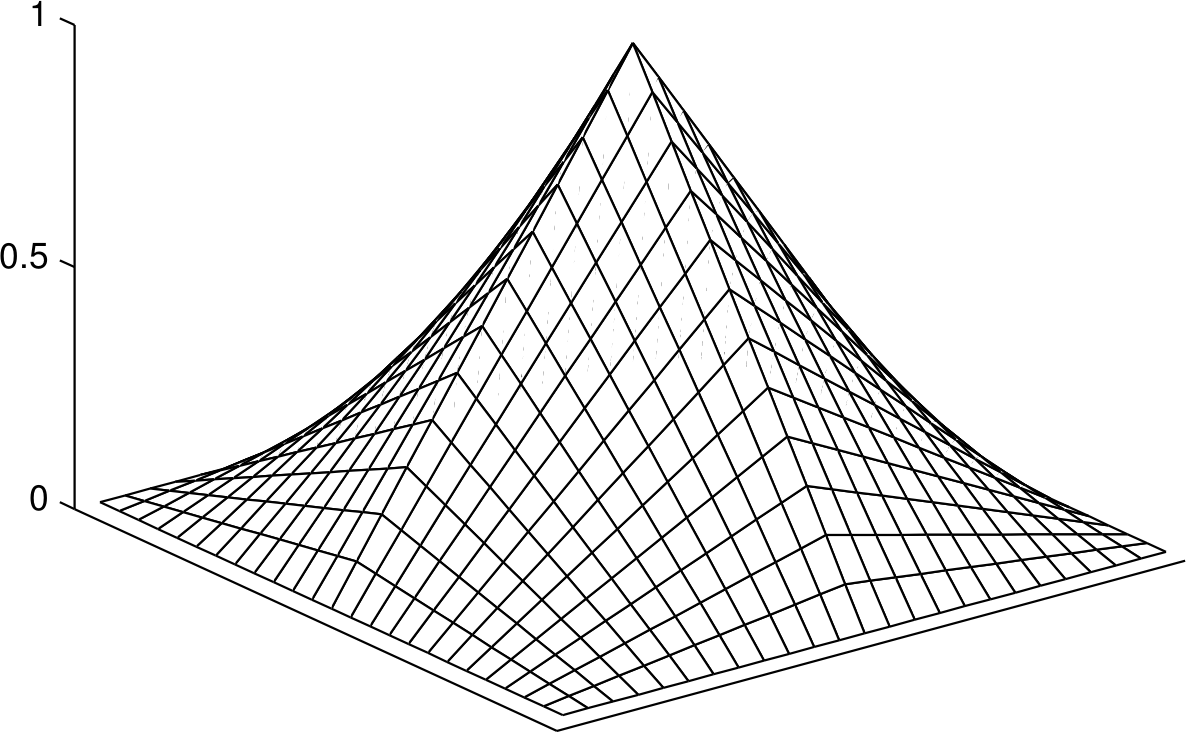
\includegraphics[width=0.35\textwidth]{figs/chapeau}
\caption{Typical $Q_1$ basis function $\phi_{ij}$.  (Figure 1.9 in \cite{Elmanetal2005}.)}
\label{fig:chapeau}
\end{figure}

The finite element solution in $u^h\in \HhD$ is a linear combination of basis functions:
\begin{equation}
	u^h(x,z) = \sum_{k,l=0}^{I,J} U_{kl} \phi_{kl}(x,z).  \label{femsolnform}
\end{equation}
The coefficients are the values at the nodes, 
\begin{equation}
    U_{kl} = u^h(x_k,z_l(x_k)).  \label{coeffsarenodevalues}
\end{equation}
Because $u^h$ satisfies the boundary conditions, we can immediately list equations for the coefficients $U_{kl}$ along boundaries I and II:
\begin{align}
  U_{k0} &= 0              &&\text{for } k=0,1,\dots,I, \label{femdirichlet} \\
  U_{0l} &= \alpha(z_l(0)) &&\text{for } l=1,\dots,J. \notag
\end{align}
The system of linear equations mostly comes from definition \eqref{femweak} using test functions which range over a basis of $\Hhzero$, however.  In fact, consider equation \eqref{femweak} for $\varphi^h = \phi_{ij}$, where $i>0$ and $j>0$, and use form \eqref{femsolnform}:
\begin{equation}
  \sum_{k,l=0}^{M,J} U_{kl} \int_\Omega \nu \left(4\frac{\partial\phi_{kl}}{\partial x} \frac{\partial\phi_{ij}}{\partial x} + \frac{\partial\phi_{kl}}{\partial z} \frac{\partial\phi_{ij}}{\partial z}\right)\dxdz = - \int_\Omega \rho g h'\,\phi_{ij} \dxdz + \int_{\mathrm{IV}} 2 \beta \phi_{ij} \,\mathrm{d}z. \label{femequation}
\end{equation}
Equation \eqref{femequation} defines one row in an $N\times N$ matrix.  Let $i>0$ and $j>0$ and define $m=n(i,j)$.  Let $k,l$ be any node of the grid and define $n=n(k,l)$.  Define
\begin{equation}
a_{mn} = \int_\Omega \nu \left(4\frac{\partial\phi_{kl}}{\partial x} \frac{\partial\phi_{ij}}{\partial x} + \frac{\partial\phi_{kl}}{\partial z} \frac{\partial\phi_{ij}}{\partial z}\right)\dxdz  \label{aintegral}
\end{equation}
and
\begin{equation}
f_m = - \int_\Omega \rho g h'\,\phi_{ij} \dxdz + \int_{\mathrm{IV}} 2 \beta \phi_{ij} \,\mathrm{d}z. \label{fintegral}
\end{equation}

The full linear system includes equations \eqref{femdirichlet} also, so that if $i=0$ or $j=0$ then $a_{mm}=1$ where $m=n(i,j)$.  In this case $f_m$ is the value of $u$ at node $i,j$, either zero or $\alpha(z_j(x_0))$.  All other entries $a_{mn}$ not covered by \eqref{femequation} or this Dirichlet case are zero.  Thus equation \eqref{femequation} determines $IJ$ equations, and equation \eqref{femdirichlet} gives an additional $I+J+1$ equations.  The total is $IJ+I+J+1=(I+1)(J+1)=N$ equations, exactly one equation for each node.  This forms the $N\times N$ system
    $$\sum_{n=1}^N  a_{mn} U_n = f_m \qquad \text{ or } \qquad A\, \mathbf{U} = \mathbf{f}.$$

\subsection*{Matrix assembly}  We must be yet more specific, however, if we want to write a program to assemble the $N\times N$ matrix $A$ and the $N\times 1$ vector $\mathbf{f}$ by local operations.

Consider integral \eqref{fintegral} to compute $f_m$, for example.  The integral over $\Omega$ is really over the support (nonzero set) of $\phi_{ij}$.  Recalling equation \eqref{phiij} and Figure \ref{fig:chapeau}, this support comes from the four quads $\square_{i-1,j-1}, \square_{i,j-1}, \square_{i,j}, \square_{i-1,j}$ which touch nodes $i,j$.

Let us change our perspective on the matrix assembly process, as follows.  Four integrations over a given quad $\quadij$ generate contributions to four different right-hand sides $f_m$.  Similarly, for integral \eqref{aintegral} we can identify and compute all the contributions to matrix entries $a_{mn}$ coming from a given quad.  On $\quadij$ there are four possible vertices at which a test function could be one and four possible vertices where the basis function $\phi_{kl}$ used in \eqref{femsolnform} could be one, so it follows that there are ten such distinct integrals over $\quadij$.  These integrals contribute to sixteen different matrix entries $a_{mn}$, but symmetrically.  Entries $a_{mn}$ and $a_{nm}$ receive the same contributions.

Fix a quad $\quadij$.  These integrals define new functions of the node indices $i,j$ and of additional vertex indices $r,s=1,2,3,4$:
\begin{align}
  X^{ij}_{rs} &= \int_{\quadij} \nu \left(4\frac{\partial\psi_{i,j,s}}{\partial x} \frac{\partial\psi_{i,j,r}}{\partial x} + \frac{\partial\psi_{i,j,s}}{\partial z} \frac{\partial\psi_{i,j,r}}{\partial z}\right)\dxdz,  \label{quadijfcns}  \\
  Y^{ij}_r    &= - \int_{\quadij} \rho g h'\,\psi_{i,j,r} \dxdz, \notag \\ 
  Z^{ij}_r    &= \begin{cases}
                    \int_{\quadij \cap \mathrm{IV}} 2 \beta \psi_{i,j,r} \,\mathrm{d}z, & i=I, \\
                    0, & \text{otherwise}.
                 \end{cases} \notag
\end{align}

To describe the actual assembly process, identifying the entries $a_{mn}$ and $f_m$ to which integrals \eqref{quadijfcns} contribute, we give the \Matlab-like pseudocode in Figure \ref{pseudoassembly}.  At each quad $\quadij$ we consider vertices $r=1,2,3,4$ in counter-clockwise order, starting with the lower-left vertex $i,j$.  At each vertex $r$ we consider the test function with value there.  From the local grid coordinates of the $r$ vertex we compute the row $m$ to which we contribute.  For $f_m$ we get the contributions $Y^{ij}_r=$ \texttt{Y(i,j,r)} and $Z^{ij}_r=$ \texttt{Z(i,j,r)} by integrations addressed in the next subsection.

For the matrix contributions we must also iterate over the solution degrees of freedom for the given quad.  We use another vertex index $s=1,2,3,4$.  Contribution $X^{ij}_{rs}=$ \texttt{X(i,j,r,s)} adds to matrix entry $a_{nm}$, where $m$ is the global index of the $r$-vertex and $n$ is the global index for the $s$-vertex.

Some additional details are worth noting:
\begin{itemize}
  \item The pseudocode assumes that there are helper functions \texttt{n(i,j)}, \texttt{alpha(j)}, \texttt{X(i,j,r,s)}, \texttt{Y(i,j,r)}, \texttt{Z(i,j,r)}, \texttt{isdirichlet(i,j)}, and \texttt{isneumannIV(i,j)}.  These are easy to implement:
    \begin{itemize}
      \item Function \texttt{n(i,j)} is equation \eqref{localtoglobal}.
      \item Functions \texttt{isdirichlet(i,j)} and \texttt{isneumannIV(i,j)} return boolean values; the former is true if $i,j$ is a node on the Dirichlet boundary I $\cup$ II, while the latter is true if $i,j$ is on the non-homogeneous Neumann boundary IV.
      \item The implementation of \texttt{X(i,j,r,s)} can enforce the symmetry $X^{ij}_{sr}=X^{ij}_{rs}$.  For example, it only does an integral in the $r\ge s$ case.
    \end{itemize}
  \item We include the Dirichlet nodes into the linear system as trivial equations, instead of eliminating them and reducing the system size, which is possible but which would obscure the assembly process.
  \item We apply Dirichlet boundary conditions so as to preserve the symmetry of $A$.  Indeed, when we come across a solution degree of freedom $s$ that corresponds to a non-homogeneous Dirichlet node (boundary component II) we immediately move its contribution over to the right-hand side using the corresponding known value $u=\alpha(z)$.
\end{itemize}

\begin{figure}
\begin{Verbatim}[xleftmargin=0.2in, frame=single, fontsize=\small]
N = (I+1)*(J+1);
A = sparse(N,N);                             % empty sparse format
b = zeros(N,1);

% easy equations for Dirichlet nodes
for i=0:I                                    % bdry I
   m = n(i,0);
   A(m,m) = 1.0;
   b(m) = 0.0;
for j=1:J                                    % bdry II
   m = n(0,j);
   A(m,m) = 1.0;
   b(m) = alpha(j);

% assembly of contributions from each quad_ij
for i = 0:I-1
   for j = 0:J-1
      ii = [i   i+1 i+1 i  ];                % traverse vertices of quad_ij
      jj = [j   j   j+1 j+1];                %    in counter-clockwise order
      for r = 1:4
         if ~isdirichlet(ii(r),jj(r))
            m = n(ii(r),jj(r));              % m = index of equation
            b(m) += Y(i,j,r);
            if isneumannIV(ii(r),jj(r))
              b(m) += Z(i,j,r);
            for s = 1:4
               X = X(i,j,r,s);
               if isdirichlet(ii(s),jj(s))   % symmetric Dirichlet
                  b(m) -= X * alpha(jj(s));
               else
                  col = n(ii(s),jj(s));      % col = index of unknown
                  A(m,col) += X;
\end{Verbatim}
\caption{Pseudocode for assembly of system $A\mathbf{U}=\mathbf{f}$.} \label{pseudoassembly}
\end{figure}

Figure \ref{fig:sparsepattern} shows the sparsity pattern generated by the pseudocode in the $I=9$ and $J=5$ case.  As noted, the pattern is symmetric.  A generic row, corresponding to a node which is not on a quad which intersects $\partial\Omega$, has nine nonzero entries from its eight grid neighbors and itself.  Consideration of the mesh shows that $2(J+2)+1$ is the expected matrix bandwidth, thus $15$ in this case.

\begin{figure}[ht] 
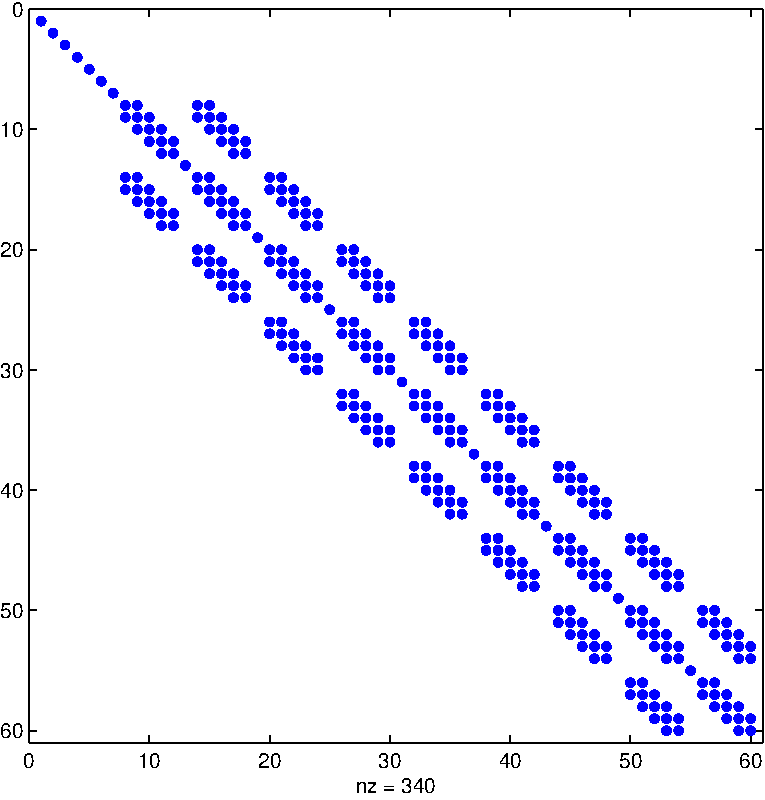
\includegraphics[width=0.45\textwidth]{figs/sparsepattern}
\caption{Sparsity pattern for matrix $A$ for same mesh shown in Figure \ref{fig:q1mesh}.}
\label{fig:sparsepattern}
\end{figure}

\newcommand{\dxidzeta}{\,\mathrm{d}\xi\,\mathrm{d}\zeta}

\subsection*{Change of variables and Gauss integration to compute the integrals}  We still do not have an implemented finite element method because integrals \eqref{quadijfcns} require actual computation.  These integrals will be referred back to a reference quad $\quadref$ using equations \eqref{quadijdefn}--\eqref{refmap}.

Recall the change-of-variables rule.  It says that for a domain $D\subset \RR^2$ and a map $F:D \to D'$ given by $F(\xi,\zeta)=(x(\xi,\zeta),z(\xi,\zeta))$, supposing $F$ is differentiable and $D'=F(D)$, we have
\begin{equation}
  \int_{D'} g(x,z)\dxdz = \int_D g(x(\xi,\zeta),z(\xi,\zeta))\,|J_F|\,\dxidzeta \label{changeofvars}
\end{equation}
for all continuous $g:D' \to \RR^2$.  By definition
	$$J_F(\xi,\zeta) = \det\,\begin{bmatrix}
	                            \frac{\partial x}{\partial \xi} & \frac{\partial z}{\partial \xi} \\
	                            \frac{\partial x}{\partial \zeta} & \frac{\partial z}{\partial \zeta}
	                          \end{bmatrix}$$
is the determinant of the Jacobian matrix, called the Jacobian determinant or just the \emph{Jacobian}.  

In our case the map is $R_{ij}:\quadref\to\quadij$ and the Jacobian $J=J_{R_{ij}}$ is computable with relative ease.  First denote the vertices of $\quadij$ as $(x^1,z^1),(x^2,z^2),(x^3,z^3),(x^4,z^4)$ using the usual lower-left-and-counter-clockwise numbering convention; compare \eqref{quadijdefn} for the actual node coordinates.  Then, recalling \eqref{chidefns} and \eqref{refmapeqns}, we compute
\begin{align*}
  \begin{bmatrix}
    \frac{\partial x}{\partial \xi} & \frac{\partial z}{\partial \xi} \\
    \frac{\partial x}{\partial \zeta} & \frac{\partial z}{\partial \zeta}
  \end{bmatrix}
&=
  \begin{bmatrix}
     \sum_{r=1}^4 x^r \frac{\partial \chi_r}{\partial \xi} & \sum_{r=1}^4 z^r \frac{\partial \chi_r}{\partial \xi} \\
	 \sum_{r=1}^4 x^r \frac{\partial \chi_r}{\partial \zeta} & \sum_{r=1}^4 z^r \frac{\partial \chi_r}{\partial \zeta}
  \end{bmatrix} \\
&= \frac{1}{4}
  \begin{bmatrix}
    (x^1 - x^2) (\zeta - 1) + (x^3 - x^4) (\zeta + 1) & (z^1 - z^2) (\zeta - 1) + (z^3 - z^4) (\zeta + 1) \\
	(x^1 - x^4) (\xi - 1) + (x^3 - x^2) (\xi + 1)     & (z^1 - z^4) (\xi - 1) + (z^3 - z^2) (\xi + 1)
  \end{bmatrix}
\end{align*}
\cite[compare (1.48)]{Elmanetal2005}.  There is a simplification in our case, however, because the grid is equally-spaced in $x$.  In fact $x^1=x_i,x^2=x_{i+1},x^3=x_{i+1},x^4=x_i$ and so $x^1-x^2=-\Delta x$, $x^3-x^4 = +\Delta x$, $x^1 - x^4 = 0$, and $x^3-x^2=0$.  Therefore
\begin{equation}
\begin{bmatrix}
    \frac{\partial x}{\partial \xi} & \frac{\partial z}{\partial \xi} \\
    \frac{\partial x}{\partial \zeta} & \frac{\partial z}{\partial \zeta}
  \end{bmatrix}
= \frac{1}{4}
  \begin{bmatrix}
    2 \Delta x & (z^1 - z^2) (\zeta - 1) + (z^3 - z^4) (\zeta + 1) \\
	0   & (z^1 - z^4) (\xi - 1) + (z^3 - z^2) (\xi + 1)
  \end{bmatrix}  \label{jacmatrix}
\end{equation}
with determinant
\begin{equation}
  J(\xi,\zeta) = \frac{1}{8} \Delta x\, \left[ (z^1 - z^4) (\xi - 1) + (z^3 - z^2) (\xi + 1)\right]. \label{jacobianij}
\end{equation}

By way of confirmation of the formulas so far, for our mesh construction note that $\quadij$ is a parallelogram if and only if $z^4-z^1=z^3-z^2$, that is, if and only if the left and right sides of the quadrilaterals have equal length.  In such a case Jacobian formula \eqref{jacobianij} simplifies to a constant $J = \Delta x\,(z^3 - z^2) / 4$, which is the ratio of the area of the parallelogram $\quadij$ to the reference quad $\quadref$.  Problem 1.7 in \cite{Elmanetal2005}, however, asserts that any parallelogram quad gives a constant Jacobian (in general).  Note that all of the quadrilaterals in our mesh are parallelograms if the glacier has constant thickness $h(x)-b(x)=H_0$.

\newcommand{\Jdd}{\,|J(\xi,\zeta)|\dxidzeta}
\newcommand{\Jpq}{J(\xi_p,\zeta_q)}

Consider integral $Y^{ij}_r$ defined in equation \eqref{quadijfcns}.  Using \eqref{psidefn} and \eqref{changeofvars} we integrate over the reference quadrilateral:
\begin{align}
  Y^{ij}_r &= -\rho g \int_{\quadij} h'(x)\,\psi_{i,j,r}(x,z) \dxdz \notag \\
           &= -\rho g \int_{-1}^1 \int_{-1}^1 h'(x(\xi,\zeta))\,\chi_r(\xi,\zeta) \Jdd. \label{integralforY}
\end{align}
The integrand in \eqref{integralforY} is fully determined by the input geometry function $h(x)$ and by additional local information about the quadrilateral $\quadij$, especially equations \eqref{chidefns} and \eqref{jacobianij}.  Note that both $x(\xi,\zeta)$ and $J(\xi,\zeta)$ depend on the particular quadrilateral, though the notation does not make this obvious.

We finally have a concrete function to integrate, but it remains too hard to do ``by hand''.\footnote{The integrand in \eqref{integralforY} is a polynomial in $\xi$ and $\zeta$, assuming a polygonal domain so that $h'$ is actually constant on (above) $\quadij$.  Similarly, integrals $X^{ij}_{rs}$ have rational integrands if $\nu(x,z)$ is rational or polynomial.  Thus these integrals \emph{could} be done exactly using antiderivatives.  Alternatively we could use sufficiently-many Gauss quadrature points so that the numerical integration is exact.}  We follow the standard approach, namely, to use Gaussian quadrature \cite[subsection 1.4.2]{Elmanetal2005}.  Among the simplest quadrature rules is the ``$m=2$'' point tensor product method used by \cite{BrownSmithAhmadia2013}.  Let $w_{pq}=1$ and let $\xi_1=\zeta_1=-\omega$ and $\xi_2=\zeta_2=+\omega$ where $\omega=1/\sqrt{3}=0.57735$ \cite[compare $m=2$ cases of Figure 1.15 and formula (1.52)]{Elmanetal2005}.  Then
\begin{equation}
  Y^{ij}_r \approx -\rho g \sum_{p=1}^2 \sum_{q=1}^2 w_{pq}\, h'(x_{pq})\,\chi_{rpq} |J_{pq}| \label{Yapprox}
\end{equation}
where $x_{pq} = x(\xi_p,\zeta_q))$, $\chi_{rpq} = \chi_r(\xi_p,\zeta_q)$, and $J_{pq}=\Jpq$.

Somewhat similar is the Neumann integral $Z^{ij}_r$ along boundary component IV.  Note $Z^{ij}_r=0$ if $i<I$, so consider cases where $i=I$.  Then for $j=0,\dots,J-1$ we have
\begin{align}
  Z^{Ij}_r &= \int_{z^2}^{z^3} 2 \beta(z) \psi_{I,j,r}(x_I,z) \,\mathrm{d}z = (z^3-z^2)\,\int_{-1}^1 \beta(z(1,\zeta)) \chi_r(1,\zeta)\, \mathrm{d}\zeta \notag \\
           &\approx (z^3-z^2)\,\sum_{p=1}^2 w_p\,\beta(z(1,\zeta_p)) \chi_r(1,\zeta_p). \label{Zapprox}
\end{align}
where, consistent with notation earlier, $z^2 = z_{j}(x_I)$ and $z^3 = z_{j+1}(x_I)$.  Also, using the calculation of $\partial z/\partial \zeta$ from \eqref{jacmatrix}, along IV we have
  $$\mathrm{d}z = \frac{\partial z}{\partial \xi}\mathrm{d}\xi + \frac{\partial z}{\partial \zeta}\mathrm{d}\zeta = \frac{\partial z}{\partial \zeta}\mathrm{d}\zeta = \frac{1}{2} (z^3-z^2)\,\mathrm{d}\zeta.$$

\newcommand{\cole}[1]{\begin{bmatrix}\frac{\partial\chi_{#1}}{\partial \xi} \\ \frac{\partial\chi_{#1}}{\partial \zeta}\end{bmatrix}}

Finally, consider the matrix contributions $X^{ij}_{rs}$.  These are more complicated, but by the same methods as above we compute
\begin{align}
  X^{ij}_{rs} &= \int_{\quadij} \nu(x,z) \left(4\frac{\partial\psi_{i,j,s}}{\partial x} \frac{\partial\psi_{i,j,r}}{\partial x} + \frac{\partial\psi_{i,j,s}}{\partial z} \frac{\partial\psi_{i,j,r}}{\partial z}\right)\dxdz \notag \\
   &= \int_{-1}^1 \int_{-1}^1 \nu(x(\xi,\zeta),z(\xi,\zeta)) \cole{s}^\top \frac{B(\xi,\zeta)}{|J(\xi,\zeta)|} \cole{r}\, \dxidzeta \label{integralforX}
\end{align}
where 
\begin{equation}
B(\xi,\zeta) = E(\xi,\zeta)^\top \begin{bmatrix} 4 & 0 \\ 0 & 1 \end{bmatrix} E(\xi,\zeta) \label{Bmatrixdefn}
\end{equation}
is a $2\times 2$ symmetric, positive-definite matrix and $E(\xi,\zeta)$ is a $2\times 2$ matrix computed by Cramer's rule:
\begin{equation}
E(\xi,\zeta) = J(\xi,\zeta)\, \begin{bmatrix}
    \frac{\partial \xi}{\partial x} & \frac{\partial \zeta}{\partial x} \\
    \frac{\partial \xi}{\partial z} & \frac{\partial \zeta}{\partial z}
  \end{bmatrix} 
  = J(\xi,\zeta)\, \begin{bmatrix}
    \frac{\partial x}{\partial \xi} & \frac{\partial z}{\partial \xi} \\
    \frac{\partial x}{\partial \zeta} & \frac{\partial z}{\partial \zeta}
  \end{bmatrix}^{-1}
  = \begin{bmatrix}
    \frac{\partial z}{\partial \zeta} & -\frac{\partial z}{\partial \xi} \\
    -\frac{\partial x}{\partial \zeta} & \frac{\partial x}{\partial \xi}
  \end{bmatrix}.   \label{Ematrixdefn}
\end{equation}
The entries of the last matrix are given by equation \eqref{jacmatrix}.

Formulas \eqref{integralforX}--\eqref{Ematrixdefn} require more explanation.  First, by equation \eqref{psidefn} we have
   $$\frac{\partial\psi_{i,j,r}}{\partial x} = \frac{\partial\psi_{i,j,r}}{\partial \xi} \frac{\partial \xi}{\partial x} + \frac{\partial\psi_{i,j,r}}{\partial \zeta} \frac{\partial \zeta}{\partial x} = \frac{\partial\chi_r}{\partial \xi} \frac{\partial \xi}{\partial x} + \frac{\partial\chi_r}{\partial \zeta} \frac{\partial \zeta}{\partial x}.$$
A similar expression applies to $\partial\psi_{i,j,r}/\partial z$.  Thus
   $$J(\xi,\zeta)\, \begin{bmatrix}
       \frac{\partial\psi_{i,j,r}}{\partial x} \\
       \frac{\partial\psi_{i,j,r}}{\partial z}
     \end{bmatrix}
  = J(\xi,\zeta)\, \begin{bmatrix}
    \frac{\partial \xi}{\partial x} & \frac{\partial \zeta}{\partial x} \\
    \frac{\partial \xi}{\partial z} & \frac{\partial \zeta}{\partial z}
  \end{bmatrix} \cole{r}
  = E\,\cole{r}.$$
On the other hand, by the chain rule $E^{-1}$ is the Jacobian matrix, so \eqref{Ematrixdefn} follows.  But the integrand for $X^{ij}_{rs}$ uses a quadratic form associated to these vectors,
	$$4\frac{\partial\psi_{i,j,s}}{\partial x} \frac{\partial\psi_{i,j,r}}{\partial x} + \frac{\partial\psi_{i,j,s}}{\partial z} \frac{\partial\psi_{i,j,r}}{\partial z} = \begin{bmatrix}
       \frac{\partial\psi_{i,j,s}}{\partial x} &
       \frac{\partial\psi_{i,j,s}}{\partial z}
     \end{bmatrix}  
     \begin{bmatrix} 4 & 0 \\ 0 & 1 \end{bmatrix} \begin{bmatrix}
       \frac{\partial\psi_{i,j,r}}{\partial x} \\
       \frac{\partial\psi_{i,j,r}}{\partial z}
     \end{bmatrix}.$$
Equations \eqref{Bmatrixdefn} and then \eqref{integralforX} follow.

Thus, using Gaussian integration, and notation just as in \eqref{Yapprox},
\begin{equation}\label{Xapprox}
	X^{ij}_{rs} \approx \sum_{p=1}^2 \sum_{q=1}^2 w_{pq}\, \nu(x_{pq},z_{pq}) \begin{bmatrix} \chi_{s;\xi,pq} \\ \chi_{s;\zeta,pq} \end{bmatrix}^\top \, \frac{B_{pq}}{ |J_{pq}|} \, \begin{bmatrix} \chi_{r;\xi,pq} \\ \chi_{r;\zeta,pq} \end{bmatrix} 
\end{equation}
where $\chi_{r;\xi,pq} = (\partial\chi_r/\partial \xi)(\xi_p,\zeta_q)$, $\chi_{r;\zeta,pq} = (\partial\chi_r/\partial \zeta)(\xi_p,\zeta_q)$ and $B_{pq}=B(\xi_p,\zeta_q)$.

The content in this subsection may look messy and complicated, but expressions \eqref{Yapprox}, \eqref{Zapprox}, and \eqref{Xapprox} are computable functions of their indices.  We are ready to write and test an actual code.


\newpage
\section{Testing in the linear case}\label{sec:linear testing}

\subsection*{Codes for linearized Blatter equation}  The previous section gave sufficient detail to build functional \Matlab/\Octave codes to solve the linearized problem.  They solve the weak form \eqref{weak}, incorporating the linearization ``fiction'' which simplifies the original equation \eqref{blatter}, and the boundary conditions shown in figure \ref{fig:bdryblatter}.  Table \ref{tab:linearcodes} lists the major components.  These, and helper components, appear in directory \texttt{mfiles/}.

\begin{table}[h]
\caption{\Matlab/\Octave codes for the linearized Blatter equation.  (Certain minor helper functions are not listed.)}
\label{tab:linearcodes}
\begin{tabular}{@{}ll}
code  & purpose/functionality \\ 
\hline
\texttt{getparams.m}\phantom{\huge h \normalsize} & physical parameters and ``typical'' values (Table \ref{tab:notation}) \\
\texttt{chifcn.m}    & evaluate $\chi_r(\xi,\zeta)$  \\
\texttt{dchifcn.m}   & evaluate $\partial\chi_r(\xi,\zeta)/\partial \xi$ and $\partial\chi_r(\xi,\zeta)/\partial \zeta$ \\
\texttt{geometry.m}  & evaluate $h(x)$, $b(x)$, $h'(x)$ \\
\texttt{vertices.m}  & compute $x_1,x_2,x_3,x_4$ and $z_1,z_2,z_3,z_4$ for $\quadij$ \\
\texttt{gaussquaddata.m} & compute $\xi_p$, $\zeta_q$, $x_{pq}$, $z_{pq}$, $J_{pq}$, $B_{pq}$  for $\quadij$ \\
\texttt{linearfem.m} & assemble $A,b$ and solve $A u = b$ using ``$A\backslash b$'' \\
\texttt{showtests.m} & generate figure \ref{fig:showtests} using \texttt{linearfem.m} \\
\texttt{verify.m}    & generate figure \ref{fig:linearverify} using \texttt{linearfem.m}
\end{tabular}
\end{table}



\subsection*{Verification}  Constants for the exact solutions FIXME

Note that the value for $B$, the ice hardness, is $1/10$th the value used in \cite{MacAyealetal}, a value thought to be appropriate for the quite cold Ross ice shelf.

\begin{table}
\caption{Parameters used in specific solutions and computations. ``Typical'' values are only used in \TESTONE and \TESTTWO.}
\label{tab:notation}
\begin{tabular}{@{}lll}
name  & meaning  & value (units) \\ 
\hline
$B$\phantom{\huge h \normalsize}     & ice hardness              & $1.9 \times 10^7$ \,(Pa s$^{1/3}$) \\
$D_0$    & typical strain rate       & $10^{-3}$  \,(a$^{-1}$) \\
$g$      & gravity                   & $9.81$     \,(m s$^{-2}$) \\
$H_0$    & typical thickness         & $1000$     \,(m) \\
$L$      & length of flow line       & $10$       \,(km) \\
$n$      & Glen exponent             & 3          \\
$\nu_0$  & typical viscosity: $2 \nu_0 = B D_0^{(1/n)-1}$ & $9.49 \times 10^{13}$ \,(Pa s) \\
$\rho$   & density of ice            & 910        \,(kg m$^{-3}$) \\
$\sigma_0$ & typical longitudinal stress at boundary & $10^5$ \,(Pa) \\
$u_0$    & typical velocity          & 20         \,(m a$^{-1}$)
\end{tabular}
\end{table}


\begin{figure}[ht] 
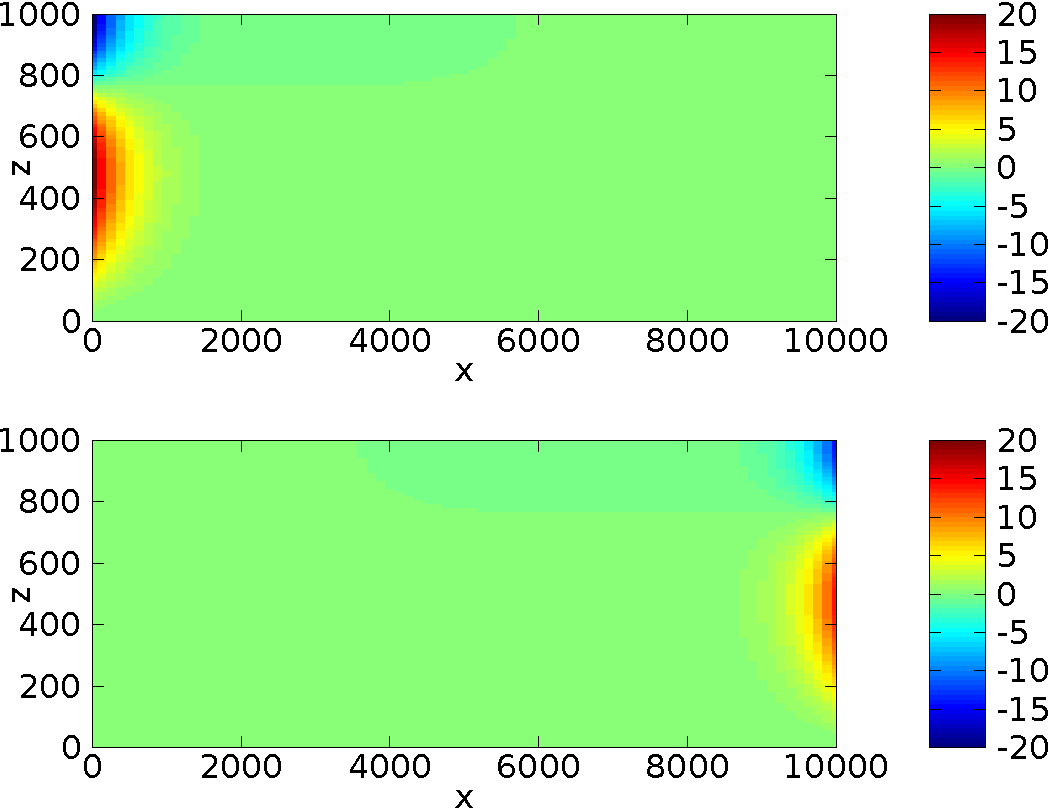
\includegraphics[width=0.65\textwidth]{figs/showtests}
\caption{Numerical solutions to \TESTONE (top) and \TESTTWO (bottom) on $I=J=80$ grids.  Exact solutions agree with these to within less than 1\% (figure \ref{fig:linearverify}), thus they would appear the same in these figures.}
\label{fig:showtests}
\end{figure}


And it works, as shown in Figure \ref{fig:linearverify}.  Note that $O(\Delta x^2)$ convergence rate is optimal for our finite element method, so at this stage we can believe the implementation.

\begin{figure}[ht] 
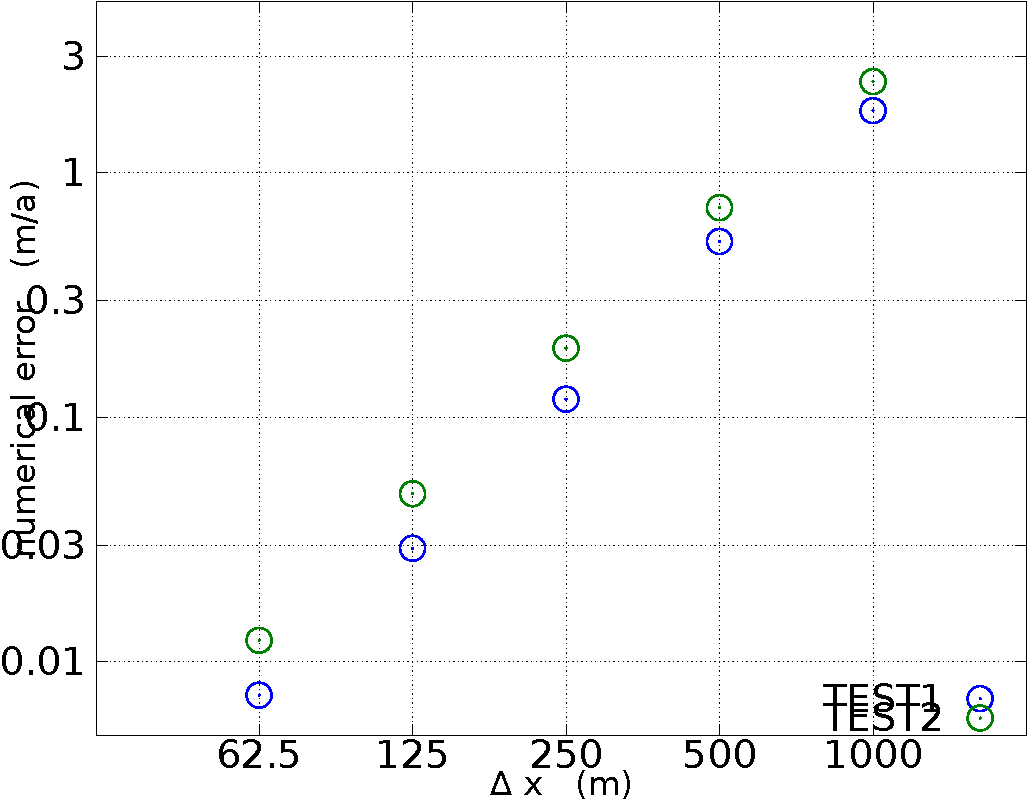
\includegraphics[width=0.6\textwidth]{figs/linearverify}
\caption{\TESTONE and \TESTTWO are used to check that we have correctly implemented the basic finite element assembly process and the nonhomogeneous boundary conditions.  Each dot on the graph is from running \texttt{linearfem.m} for a problem in Exercise B.1, comparing to the exact solution to that problem by measuring the $L^\infty$ norm; see text.  Convergence is measured to be at rates $O(\Delta x^{2.006})$ and $O(\Delta x^{1.907})$ for \TESTONE and \TESTTWO, respectively.}
\label{fig:linearverify}
\end{figure}


\clearpage
\newpage
\section{Newton method for the nonlinearity}\label{sec:nonlinear}  The problem solved in the previous section is not yet the Blatter model \eqref{blatter}, which is nonlinear.  Indeed, with the ``fiction'' adopted in section \ref{sec:continuum}, the problem is a linear PDE.  It has these nontrivial features which distinguish it from a textbook Poisson problem:
\begin{itemize}
\item a generally non-constant coefficient $\nu(x,z)$,
\item a region which is determined by glacier geometry $h(x)$ and $b(x)$, and
\item a weak form equation \eqref{weak} which has ``$(4u_x,u_z)$'' instead of the gradient ``$(u_x,u_z)$''.
\end{itemize}

It remains to incorporate the nonlinear dependence of the (regularized) viscosity on the strain rates, namely to include equation \eqref{viscreg} in the Blatter equation \eqref{blatter}.  Fortunately, the derivation in section  \ref{sec:continuum} of the linearized weak form \eqref{weak} works for the nonlinear Blatter equation as well, once the correct function spaces are identified.  Indeed, the following definitions are found in \cite{RappazReist05,SchoofCoulombBlatter}, applying to the nonsliding case and flowline geometry.  Specifically, the weak form below is equation (2.6) in \cite{RappazReist05}, and it is also the case of plastic till with large yield stress ($\tau_c=|\Sigma_i^t|$ large for every $\mathbf{u}$ in equation (2.8a)) in \cite{SchoofCoulombBlatter}.

\begin{defn}  Let $p=1+1/n$.  The normed vector space $\X=\Wonep$ consists of all functions $f : \Omega \to \RR$ for which \cite{Evans}
	$$\|f\|_X = \left(\int_\Omega |f|^p + |f_x^2 + f_z^2|^{p/2} \dxdz\right)^{1/p} < \infty.$$
The \emph{solution (trial)} space $X_D$ and \emph{test} space $X_0$ are subsets of $\X$, namely
     $$X_D = \left\{f \in \X \,\Big|\, f|_{I} = 0, f|_{II} = \alpha(x)\right\}, \qquad X_0 = \left\{f \in \X \,\Big|\, f|_{I} = 0, f|_{II} = 0\right\}.$$
A function $u=u(x,z)\in \XD$ \emph{solves the weak form} of equation \eqref{blatter} if
\begin{equation}
\int_\Omega \nu\, (4 u_x, u_z) \cdot \nabla \varphi \dxdz = - \int_\Omega \rho g h'\,\varphi \dxdz + \int_{\mathrm{IV}} 2 \beta \varphi \,\mathrm{d}z \label{weakfull}
\end{equation}
for all $\varphi=\varphi(x,z)\in \Xzero$, where $\nu = \nu(u_x,u_z)$ is given by equation \eqref{viscreg}, namely
     $$\nu = \frac{B_0}{2} \left(u_x^2 + \frac{1}{4}u_z^2 + \eps_0^2\right)^{(p-2)/2}$$
noting $p-2 = (1-n)/n$.
\end{defn}

Note that Glen power law ice rheology with $1<n<\infty$ corresponds to $1<p<2$.  The typical glaciological case $n=3$ is $p=4/3$.

FIXME:  Picard has been used a lot, e.g.~\cite{Pattyn03}, but Brown and others \cite{BrownSmithAhmadia2013} use Newton, which is what we do next.

\subsection*{Newton's iterative scheme, for nonlinear viscosity}  We consider the discrete problem to be in the very general form
\begin{equation}
   \bbF(\bU) = 0.  \label{abstract}
\end{equation}
The function $\bbF(\bU)$ denotes $N$ scalar, differentiable functions of $N$ variables,
	$$\bbF(\bU)=\{f_i(U_1,\dots,U_N)\}_{i=1,\dots,N}.$$
The components $f_i$ are called \emph{residuals} or \emph{residual functions}, in the sense that nonzero outputs from these functions imply \eqref{abstract} has not been solved by their input $\bU$.

Newton's method \cite[subsection 9.6]{Pressetal} is a well-known iterative technique for solving such systems of equations.  It works if the residuals are sufficiently differentiable functions and the if the initial iterate is sufficiently close to the desired solution \cite{BurdenFaires}.  It is usually written in ``update'' form, as follows, in which we solve a linear system for the step $\bs$ and then update the approximate solution:
\begin{gather}
J(\bU_n)\, \bs = - \bbF(\bU_n), \label{newtonstep} \\
\bU_{n+1} = \bU_n + \bs \notag
\end{gather}
For each candidate solution $\bU$, the \emph{Jacobian} $J(\bU)$ is an $N\times N$ matrix with entries
\begin{equation} \label{jacobiandefn}
J(\bU)_{ij} = \frac{\partial f_i}{\partial U_j}.
\end{equation}

Form \eqref{newtonstep} of Newton's method may not be familiar from calculus.  If we were solving a scalar problem $f(u)=0$, however, then we might write the linearization $\ell(u)=f(u_n) + f'(u_n)(u-u_n)$ and then the Newton step as $\ell(u_{n+1}) = f(u_n) + f'(u_n) (u_{n+1}-u_n) = 0$, which is the same as $f'(u_n) (u_{n+1} - u_n) = -f(u_n)$, which is the direct analog of \eqref{newtonstep}.

Newton's method comes with few guarantees but it generates fast convergence.  It is generally not globally-convergent because for some starting points the method may not converge to anything, and for others it may converge to values which are not a solution of the equations.  There are, however, robust ``globalization'' techniques which greatly improve this aspect and make Newton's method very practical \cite[subsection 9.7]{Pressetal}.   The key advantage of Newton's method is that it is quadratically-convergent once iterates are close to a solution at which the residual function is twice differentiable \cite{BurdenFaires}.  Properly-globalized Newton's method is known to work quickly on many nonlinear PDE problems, as long as good information is available to inform a choice of initial guess, as long as attention is paid to how the Jacobian is extracted and to the way the linear problem for the Newton step is solved.

\subsection*{Jacobian evaluation}  We regard continuum Equation \eqref{weakfull} as a nonlinear equation ``$\bbF(\bU)=0$'' to be solved by Newton's method.  Notation is useful in constructing the Jacobian, however.  First define
	$$M = \begin{pmatrix} 4 & 0 \\ 0 & 1 \end{pmatrix}, \qquad H(t) = \frac{B_0}{2} \left(\frac{1}{4} t + \eps_0^2\right)^{(p-2)/2}.$$
Now, for fixed $\varphi\in X_0$, and $u\in X_D$ denoting either the exact solution or an approximation of it, define
	$$F_0(u) = \int_\Omega H(\grad u^\top M \grad u) \,\Big(\grad u^\top M \grad \varphi\Big) \dxdz,$$
where
    $$\grad u = \begin{pmatrix} u_x \\ u_z \end{pmatrix}, \qquad \grad \varphi = \begin{pmatrix} \varphi_x \\ \varphi_z \end{pmatrix}$$
are rcolumn vectors.  Note $H(t)$ is evaluated at
	$$t = t(u) = \grad u^\top M \grad u = \begin{pmatrix} u_x &  u_z \end{pmatrix} \begin{pmatrix} 4 & 0 \\ 0 & 1 \end{pmatrix} \begin{pmatrix} u_x \\ u_z \end{pmatrix} = 4 u_x^2 + u_z^2$$
when computing the viscosity.  Finally define
	$$G = - \int_\Omega \rho g h'\,\varphi \dxdz + \int_{\mathrm{IV}} 2 \beta \varphi \,\mathrm{d}z.$$
Then the weak form \eqref{weakfull} says that $u\in X_D$ satisfies
\begin{equation}\label{continuumF}
	F(u) = F_0(u) - G = 0
\end{equation}
for this particular $\varphi\in X_0$.

To compute the Jacobian we must differentiate $F_0$.  In fact, let $s\in X_0$ be the Newton step, so that $u+s \in X_D$ if $u\in X_D$.  Furthermore,
	$$J(u) s = F(u+s) - F(u) + O(\|s\|^2) = F_0(u+s) - F_0(u) + O(\|s\|^2).$$
On the other hand,
\begin{align*}
  H([\grad u+\grad s]^\top M [\grad u+\grad s]) &= H(t + 2 \grad u^\top M \grad s + \eps) \\
      &=  H(t) + H'(t) (2 \grad u^\top M \grad s + \eps) + \eps \\
      &=  H(t) + 2 H'(t) (\grad u^\top M \grad s) + \eps
\end{align*}
where, at each stage, ``$\eps$'' denotes a small quantity in the size of the step, $\eps = O(|\grad s|^2)$.  The derivative of $H(t)$ is just calculus,
   $$H'(t) = \frac{B_0(p-2)}{16} \left(\frac{1}{4} t + \eps_0^2\right)^{(p-4)/2}.$$
Thus we compute
\begin{align*}
  F_0(u+s) &= \int_\Omega H([\grad u+\grad s]^\top M [\grad u+\grad s]) \,\Big([\grad u+\grad s]^\top M \grad \varphi\Big)\dxdz \\
           &= \int_\Omega \left\{H(t) + 2 H'(t) (\grad u^\top M \grad s) + \eps\right\} \,\Big([\grad u+\grad s]^\top M \grad \varphi\Big)\dxdz \\
           &= F_0(u) + \int_\Omega H(t) \,\Big(\grad s^\top M \grad \varphi\Big)\dxdz \\
           &\qquad\qquad + \int_\Omega 2 H'(t) \,\Big(\grad u^\top M \grad s\Big) \,\Big(\grad u^\top M \grad \varphi\Big)\dxdz + O(\|s\|^2).
\end{align*}
By symmetry of $M$ it follows that
\begin{equation}
  J(u) s = \int_\Omega \left\{H(t) \,\grad \varphi + 2 H'(t) \,\Big(\grad u^\top M \grad \varphi\Big) \, \grad u\right\}^\top M \grad s \dxdz.  \label{continuumjacobian}
\end{equation}


\subsection*{Algorithm} 



\newpage
\section{Comparison to SIA velocity field}\label{sec:sia}

Before comparing velocity fields let us recall how the vertical component is found.  Because only basal boundary condition and incompressibility are used, the computation of the vertical component $w(x,z)$ is common to all shallow theories in which the horizontal component is found through a well-posed problem.  Indeed, there is no need in the Blatter model, or the shallower SIA and SSA models either, to consider the vertical velocity $w$ until after we have computed the horizontal velocity $u=u(x,z)$ from the geometry and the ice hardness.

Recall that incompressibility is $u_x + w_z = 0$ in the flowline case.  Because we assume there is no slip at the base, it follows that the vertical velocity is found from the integral
\begin{equation}
w(x,z) = - \int_{b(x)}^z u_x(x,\zeta)\,d\zeta. \label{incomp}
\end{equation}
Another important quantity, related especially to the mass continuity equation, is the horizontal flux of ice
\begin{equation}
q(x) = \int_{b(x)}^{h(x)} u(x,z)\,dz.\label{flux}
\end{equation}

We wish to compare the Blatter and SIA models.  If we compare the horizontal velocity $u(x,z)$, the vertical velocity $w(x,z)$, and the flux $q(x)$ from these two models then we are really comparing different measures of the horizontal velocity $u$.


\newpage
\section{Conclusion}  The method we have used is meant to be effective for whole ice sheet problems.  Indeed, Brown and others \cite{BrownSmithAhmadia2013} show that this method can be implemented in parallel to be many times faster than previous methods and to be weakly-scalable in the sense that more parallel processors can handle proportionally finer grids in the same amount of time.  FIXME: complete

\newpage
\bibliography{ice-bib}
\bibliographystyle{siam}



\appendix

\newpage
\section{Stress-free upper-surface boundary condition details}  The upper surface sees a balance of normal forces between that exerted by the ice fluid and that exerted by the atmosphere.  If $\mathbf{n}$ is an upward normal vector at the surface then the normal force from the ice is $\sigma_{ij} n_j$ if $\sigma_{ij}$ is the Cauchy stress tensor.  The normal force from the air is $-p_{\text{atm}} n_j$.  These sum to zero, that is, $\sigma_{ij} n_j = p_{\text{atm}} n_j$

The deviatoric stress $\tau_{ij}$ and the ice fluid pressure $p$ are defined by decomposing the Cauchy stress tensor to remove its trace: $\sigma_{ij} = \tau_{ij} - p \delta_{ij}$, $\tau_{ii}=0$ \cite[equation (3.133); note summation convention]{GreveBlatter2009}.  In our flowline situation with upward normal $\mathbf{n}=(-h',1)$, and with the approximation $p_{\text{atm}}\approx 0$ which we adopt from now on, the force balance condition at the surface is equivalent to the pair \cite[equations (2.9) and (2.10)]{SchoofHindmarsh}:
\begin{align}
(p - \tau_{11})h' + \tau_{13} &= 0 \label{upperwithp}\\
-p - \tau_{11} - \tau_{13} h' &= 0. \notag
\end{align}
Equations \eqref{upperwithp} are part of the Stokes model, and have no shallow approximation.  In deriving these equations we note that by symmetry in the $y$-direction, $\tau_{11},\tau_{13},\tau_{31},\tau_{33}$ are the only nonzero components of the deviatoric tensor, also that $\tau_{31}=\tau_{13}$, and also that by incompressibility and the flow law, $\tau_{11}=\tau_{33}$.

Schoof \& Hindmarsh \cite{SchoofHindmarsh} apply a scaling argument to the flow line Stokes model to get the Blatter model.  Their scaling uses independent dimensionless parameters $\eps = [H]/[x], \lambda = [\tau_{13}]/[\tau_{11}]$ where $[H]$ is a typical thickness, $[x]$ is the horizontal length scale, and $[\tau_{13}],[\tau_{11}]$ are typical scales for stresses.  Heuristically, $\eps$ is a shallowness ratio, and should be small when the Blatter model is applied, while $\lambda$ can be thought of as a measure of slip.  Note that $\lambda$ is part of the scaling, but \emph{it is not small}; the point of the study in \cite{SchoofHindmarsh} is to show that the Blatter model applies for all cases $\lambda \ll 1$, $\lambda = O(1)$, $\lambda \gg 1$.

When scaled this way, equations \eqref{upperwithp} become
\newcommand{\eol}{\frac{\eps}{\lambda}}
\begin{align}
(p - \eol \tau_{11})h' + \tau_{13} &= 0 \label{scaledupperwithp}\\
-p - \eol \tau_{11} - \eps^2 \tau_{13} h' &= 0. \notag
\end{align}
Compare \cite[equations (2.29) and (2.30)]{SchoofHindmarsh}.  From the second of these equations we see that, up to $O(\eps^2)$ terms which are dropped throughout the Blatter model, $p = - (\eps/\lambda) \tau_{11}$.  Thus we can eliminate the ice pressure $p$ at the surface.  We see that equations \eqref{scaledupperwithp} are equivalent to the single equation
\begin{equation}
- 2 \eol \tau_{11} h' + \tau_{13} = 0. \label{droppedupper}
\end{equation}

On the other hand, up to error $O(\eps^2)$ terms which are dropped, $u_x = Z \tau_{11}$ and $u_z = 2 \eps\lambda Z \tau_{13}$, where $Z=(\tau_{11}^2+\lambda^2\tau_{13}^2)^{(n-1)/2}$.  We can now write equation \eqref{droppedupper} in terms of $u$, immediately dropping a common factor $Z$, to get
   $$- 2 \eol u_x h' + \frac{1}{2\eps\lambda} u_z = 0.$$
Multiplying through by $2\eps\lambda$ gives and equation without the scaling parameter $\lambda$,
\begin{equation}
- 4 \eps^2 u_x h' + u_z = 0.  \label{sweet}
\end{equation}
Returning to dimensional coordinates gives \eqref{upper}.  This is the upper surface condition stated by Pattyn \cite{Pattyn03} and Rappaz and Reist \cite{RappazReist05}, and as used without explanation by Brown et al.~\cite{BrownSmithAhmadia2013}.


\newpage
\section{Exercises}

\renewcommand{\labelenumi}{\emph{\alph{enumi})}\quad}
\subsection{Exercise}  \label{exer:constantseparable}  Exact solutions of PDEs are useful to eliminate all coding errors in the implementation of a finite element method.  For such purposes here, consider a flat bed $b(x)=0$ and constant thickness $h(x)=H_0$, so that our domain $\Omega$ (see equation \eqref{domain}) is a rectangle and the right-hand side of equation \eqref{blatter} is zero.  Suppose that instead of \eqref{visc}, we simply assume that the viscosity is constant, $\nu(x,z)=\nu_0$.  In this simplest test case we can find PDE solutions by hand using classical separation of variables techniques, as in \cite{BrownChurchill} for example.  The main text, and the next exercise, then illustrate the \emph{use} of these solutions to verify numerics.
\begin{enumerate}
\item Supposing zero downstream stress, $\beta(z)=0$ in \eqref{downstream}, show that all separable solutions of the form $u(x,z)=X(x)Z(z)$, solving equation \eqref{blatter} and homogeneous boundary conditions I, III, and IV,  are $u(x,z) = A \cosh(\lambda_k (x-L)) \sin(2 \lambda_k z)$ where $\lambda_k = (2k+1)\pi / (4 H_0)$ and $k$ is an integer.  Show that this solution $u(x,z)$ also satisfies boundary condition I if, for a concrete case, we choose $k=1$, $A=u_0/\cosh(\lambda_1 L)$, and $\alpha(z)=u_0 \sin(2 \lambda_1 z)$ where $u_0$ is a horizontal velocity scale.  This defines \TESTONE.
\item Now suppose zero upstream velocity, $\alpha(z)=0$.  Show that all separable solutions $u(x,z)=X(x)Z(z)$, solving \eqref{blatter} and boundary conditions I, II, and III, are $u(x,z) = B \sinh(\lambda_k x) \sin(2 \lambda_k z)$ for the same eigenvalues $\lambda_k$ in part \emph{a)}.  For a concrete case, again consider $k=1$ and set $B=\sigma_0 \left(\lambda_1 \cosh(\lambda_1 L) \nu_0\right)^{-1}$ where $\sigma_0$ is a stress scale.  Show that this solution satisfies boundary condition IV with $\beta(z) = 2 \sigma_0 \sin(2 \lambda_1 z)$.  This defines \TESTTWO.
\end{enumerate}

\subsection{Exercise}
\begin{enumerate}
\item  Using glaciologically-vaguely-reasonable values for $L,H_0,\nu_0,u_0,\sigma_0$ from Table \ref{tab:notation}, use Matlab to plot the exact solutions \TESTONE, \TESTTWO in parts \emph{a)} and \emph{b)}, respectively.  That is, generate Figure \ref{fig:showtests}.  Note that these solutions suggest that even for a glacier with a 1/10 aspect ratio, and even with rather soft ``ice'', the influence of longitudinal stresses penetrates not very far into the ice, in this nonsliding case.
\item Use \texttt{linearfem.m}, on refining grids with  $I=J=5,10,20,40,80$ but $\gamma=1.5$ fixed, on the concrete cases addressed in Exercise \ref{exer:constantseparable}, to reproduce Figure \ref{fig:linearverify}.
\end{enumerate}

\end{document}
